\hypertarget{summary}{%
\section{Summary}\label{summary}}

This article presents \href{https://perso.crans.org/besson/}{my}
numerical environment \emph{SMPyBandits}, written in
\href{https://www.python.org/}{Python (2 or 3)} {[}@python{]}, for
numerical simulations on \emph{single}-player and \emph{multi}-players
\href{https://en.wikipedia.org/wiki/Multi-armed_bandit}{Multi-Armed
Bandits (MAB)} algorithms {[}@Bubeck12{]}.

\emph{SMPyBandits} is the most complete open-source implementation of
state-of-the-art algorithms tackling various kinds of sequential
learning problems referred to as Multi-Armed Bandits. It aims at being
extensive, simple to use and maintain, with a clean and perfectly
documented codebase. But most of all it allows fast prototyping of
simulations and experiments, with an easy configuration system and
command-line options to customize experiments while starting them (see
below for an example).

\emph{SMPyBandits} does not aim at being blazing fast or perfectly
memory efficient, and comes with a pure Python implementation with no
dependency except standard open-source Python packages. Even if some
critical parts are also available as a \texttt{C} Python extension, and
even by using Numba {[}@numba{]} whenever it is possible, if simulation
speed really matters, one should rather refer to less exhaustive but
faster implementations, like for example {[}@TorLibbandit{]} in
\texttt{C++} or {[}@VishMABjl{]} in Julia.

\begin{center}\rule{0.5\linewidth}{\linethickness}\end{center}

\hypertarget{presentation}{%
\subsection{Presentation}\label{presentation}}

\hypertarget{single-player-mab}{%
\subsubsection{Single-Player MAB}\label{single-player-mab}}

Multi-Armed Bandit (MAB) problems are well-studied sequential decision
making problems in which an agent repeatedly chooses an action (the
``arm'' of a one-armed bandit) in order to maximize some total reward
{[}@Robbins52,LaiRobbins85{]}. Initial motivation for their study came
from the modeling of clinical trials, as early as 1933 with the seminal
work of Thompson {[}@Thompson33{]}. In this example, arms correspond to
different treatments with unknown, random effect. Since then, MAB models
have been proved useful for many more applications, that range from
cognitive radio {[}@Jouini09{]} to online content optimization (news
article recommendation {[}@Li10{]}, online advertising
{[}@LiChapelle11{]} or A/B Testing {[}@Kaufmann14;Jamieson17{]}), or
portfolio optimization {[}@Sani12{]}.

This Python package is the most complete open-source implementation of
single-player (classical) bandit algorithms
(\href{https://smpybandits.github.io/docs/Policies.html}{over 65!}). We
use a well-designed hierarchical structure and
\href{https://smpybandits.github.io/uml_diagrams/README.html}{class
inheritance scheme} to minimize redundancy in the codebase, and for
instance the code specific to the UCB algorithm
{[}@LaiRobbins85;@Auer02{]} is as short as this (and fully documented),
by inheriting from the
\href{https://smpybandits.github.io/docs/Policies.IndexPolicy.html}{\texttt{IndexPolicy}}
class:

\begin{Shaded}
\begin{Highlighting}[]
\ImportTok{from}\NormalTok{ numpy }\ImportTok{import}\NormalTok{ sqrt, log}
\ImportTok{from}\NormalTok{ .IndexPolicy }\ImportTok{import}\NormalTok{ IndexPolicy}

\KeywordTok{class}\NormalTok{ UCB(IndexPolicy):}
  \CommentTok{""" The UCB policy for bounded bandits.}
\CommentTok{  Reference: [Lai & Robbins, 1985]. """}

  \KeywordTok{def}\NormalTok{ computeIndex(}\VariableTok{self}\NormalTok{, arm):}
    \CommentTok{r""" Compute the current index, at time t and}
\CommentTok{    after :math:`N_k(t)` pulls of arm k:}

\CommentTok{    .. math::}

\CommentTok{        I_k(t) = \textbackslash{}frac\{X_k(t)\}\{N_k(t)\}}
\CommentTok{        + \textbackslash{}sqrt\{\textbackslash{}frac\{2 \textbackslash{}log(t)\}\{N_k(t)\}\}.}
\CommentTok{    """}
    \ControlFlowTok{if} \VariableTok{self}\NormalTok{.pulls[arm] }\OperatorTok{<} \DecValTok{1}\NormalTok{:  }\CommentTok{# forced exploration}
      \ControlFlowTok{return} \BuiltInTok{float}\NormalTok{(}\StringTok{'+inf'}\NormalTok{)   }\CommentTok{# in the first steps}
    \ControlFlowTok{else}\NormalTok{:                    }\CommentTok{# or compute UCB index}
\NormalTok{      estimated_mean }\OperatorTok{=}\NormalTok{ (}\VariableTok{self}\NormalTok{.rewards[arm] }\OperatorTok{/} \VariableTok{self}\NormalTok{.pulls[arm])}
\NormalTok{      exploration_bias }\OperatorTok{=}\NormalTok{ sqrt((}\DecValTok{2} \OperatorTok{*}\NormalTok{ log(}\VariableTok{self}\NormalTok{.t)) }\OperatorTok{/} \VariableTok{self}\NormalTok{.pulls[arm])}
      \ControlFlowTok{return}\NormalTok{ estimated_mean }\OperatorTok{+}\NormalTok{ exploration_bias}
\end{Highlighting}
\end{Shaded}

\hypertarget{multi-players-mab}{%
\subsubsection{Multi-Players MAB}\label{multi-players-mab}}

For Cognitive Radio applications, a well-studied extension is to
consider \(M\geq2\) players, interacting on the \emph{same} \(K\) arms.
Whenever two or more players select the same arm at the same time, they
all suffer from a collision. Different collision models has been
proposed, and the simplest one consist in giving a \(0\) reward to each
colliding players. Without any centralized supervision or coordination
between players, they must learn to access the \(M\) best resources
(\emph{i.e.}, arms with highest means) without collisions.

This package implements
\href{https://smpybandits.github.io/docs/Environment.CollisionModels.html}{all
the collision models} found in the literature, as well as all the
algorithms from the last 10 years or so (including
\href{https://smpybandits.github.io/docs/PoliciesMultiPlayers.rhoRand.html}{\texttt{rhoRand}}
from 2009,
\href{https://smpybandits.github.io/docs/Policies.MEGA.html}{\texttt{MEGA}}
from 2015,
\href{https://smpybandits.github.io/docs/Policies.MusicalChair.html}{\texttt{MusicalChair}}
from 2016, and our state-of-the-art algorithms
\href{https://smpybandits.github.io/docs/PoliciesMultiPlayers.RandTopM.html}{\texttt{RandTopM}}
and
\href{https://smpybandits.github.io/docs/PoliciesMultiPlayers.MCTopM.html}{\texttt{MCTopM}})
from {[}@BessonALT2018{]}.

\begin{center}\rule{0.5\linewidth}{\linethickness}\end{center}

\hypertarget{purpose}{%
\subsection{Purpose}\label{purpose}}

The main goal of this package is to implement
\href{https://smpybandits.github.io/API.html}{with the same API} most of
the existing single- and multi-player multi-armed bandit algorithms.
Each algorithm comes with a clean documentation page, containing a
reference to the research article(s) that introduced it, and with
remarks on its numerical efficiency.

It is neither the first nor the only open-source implementation of
multi-armed bandits algorithms, although one can notice the absence of
any well-maintained reference implementation. I built \emph{SMPyBandits}
from a framework called \emph{pymaBandits} {[}@pymaBandits{]}, which
implemented a few algorithms and three kinds of arms, in both Python and
MATLAB. The goal was twofolds, first to implement as many algorithms as
possible to have a complete implementation of the current state of
research in MAB, and second to implement multi-players simulations with
different models.

Since November \(2016\), I follow actively the latest publications
related to Multi-Armed Bandits (MAB) research, and usually I implement
quickly any new algorithms. For instance,
\href{https://smpybandits.github.io/docs/Policies.Exp3PlusPlus.html}{Exp3++},
\href{https://smpybandits.github.io/docs/Policies.CORRAL.html}{CORRAL}
and
\href{https://smpybandits.github.io/docs/Policies.SparseUCB.html}{SparseUCB}
were each introduced by articles
(\href{https://arxiv.org/pdf/1702.06103}{for Exp3++},
\href{https://arxiv.org/abs/1612.06246v2}{for CORRAL},
\href{https://arxiv.org/abs/1706.01383}{for SparseUCB}) presented at
COLT in July 2017,
\href{https://smpybandits.github.io/docs/Policies.LearnExp.html}{LearnExp}
comes from a \href{https://arxiv.org/abs/1702.04825}{NIPS 2017 paper},
and
\href{https://smpybandits.github.io/docs/Policies.klUCBPlusPlus.html}{kl-UCB++}
from an \href{https://hal.inria.fr/hal-01475078}{ALT 2017 paper}.

\begin{center}\rule{0.5\linewidth}{\linethickness}\end{center}

\hypertarget{features}{%
\subsection{Features}\label{features}}

With this numerical framework, simulations can run on a single CPU or a
multi-core machine using joblib {[}@joblib{]}, and summary plots are
automatically saved as high-quality PNG, PDF and EPS (ready for being
used in research article), using matplotlib {[}@matplotlib{]} and
seaborn {[}@seaborn{]}. Making new simulations is very easy, one only
needs to write a configuration script and no knowledge of the internal
code architecture.

\hypertarget{examples-of-configuration-for-some-simulations}{%
\subsubsection{Examples of configuration for some
simulations}\label{examples-of-configuration-for-some-simulations}}

A small script
\href{https://smpybandits.github.io/docs/configuration.html}{\texttt{configuration.py}}
is used to import the
\href{https://smpybandits.github.io/docs/Arms.html}{arm classes}, the
\href{https://smpybandits.github.io/docs/Policies.html}{policy classes}
and define the problems and the experiments. For instance, we can
compare the standard anytime
\href{https://smpybandits.github.io/docs/Policies.klUCB.html}{\texttt{klUCB}}
algorithm against the non-anytime variant
\href{https://smpybandits.github.io/docs/Policies.klUCBPlusPlus.html}{\texttt{klUCBPlusPlus}}
algorithm, as well as
\href{https://smpybandits.github.io/docs/Policies.UCBalpha.html}{\texttt{UCB}}
(with \(\alpha=1\)) and
\href{https://smpybandits.github.io/docs/Policies.Thompson.html}{\texttt{Thompson}}
(with
\href{https://smpybandits.github.io/docs/Policies.Posterior.Beta.html}{Beta
posterior}). See below in Figure \ref{fig:plot1} for the result showing
the average regret for these \(4\) algorithms.

\begin{Shaded}
\begin{Highlighting}[]
\ImportTok{from}\NormalTok{ Arms }\ImportTok{import} \OperatorTok{*;}  \ImportTok{from}\NormalTok{ Policies }\ImportTok{import} \OperatorTok{*}

\NormalTok{configuration }\OperatorTok{=}\NormalTok{ \{}
  \StringTok{"horizon"}\NormalTok{: }\DecValTok{10000}\NormalTok{,     }\CommentTok{# Finite horizon of the simulation}
  \StringTok{"repetitions"}\NormalTok{: }\DecValTok{1000}\NormalTok{,  }\CommentTok{# Number of repetitions}
  \StringTok{"n_jobs"}\NormalTok{: }\DecValTok{-1}\NormalTok{,         }\CommentTok{# Max number of cores for parallelization}
  \CommentTok{# Environment configuration, you can set up more than one.}
  \StringTok{"environment"}\NormalTok{: [ \{}
      \StringTok{"arm_type"}\NormalTok{: Bernoulli,}
      \StringTok{"params"}\NormalTok{: [}\FloatTok{0.1}\NormalTok{, }\FloatTok{0.2}\NormalTok{, }\FloatTok{0.3}\NormalTok{, }\FloatTok{0.4}\NormalTok{, }\FloatTok{0.5}\NormalTok{, }\FloatTok{0.6}\NormalTok{, }\FloatTok{0.7}\NormalTok{, }\FloatTok{0.8}\NormalTok{, }\FloatTok{0.9}\NormalTok{]}
\NormalTok{  \}],}
  \CommentTok{# Policies that should be simulated, and their parameters.}
  \StringTok{"policies"}\NormalTok{: [}
\NormalTok{      \{}\StringTok{"archtype"}\NormalTok{: klUCB, }\StringTok{"params"}\NormalTok{: \{\} \},}
\NormalTok{      \{}\StringTok{"archtype"}\NormalTok{: klUCBPlusPlus,}
       \StringTok{"params"}\NormalTok{: \{ }\StringTok{"horizon"}\NormalTok{: }\DecValTok{10000}\NormalTok{ \} \},}
\NormalTok{      \{}\StringTok{"archtype"}\NormalTok{: UCBalpha,}
       \StringTok{"params"}\NormalTok{: \{ }\StringTok{"alpha"}\NormalTok{: }\DecValTok{1}\NormalTok{ \} \},}
\NormalTok{      \{}\StringTok{"archtype"}\NormalTok{: Thompson, }\StringTok{"params"}\NormalTok{: \{\} \},}
\NormalTok{  ]\}}
\end{Highlighting}
\end{Shaded}

For a second example, this snippet is a minimal example \footnote{See
  the file
  \href{https://smpybandits.github.io/docs/configuration_multiplayers.html}{\texttt{configuration\_multiplayers.py}}
  in the code for more details.} of configuration for multiplayer
simulations, comparing different multi-player algorithms used with the
\href{https://smpybandits.github.io/docs/Policies.klUCB.html}{\texttt{klUCB}}
index policy. See below in Figure \ref{fig:plot2} for an illustration.

\begin{Shaded}
\begin{Highlighting}[]
\ImportTok{from}\NormalTok{ Arms }\ImportTok{import} \OperatorTok{*;}  \ImportTok{from}\NormalTok{ Policies }\ImportTok{import} \OperatorTok{*}
\ImportTok{from}\NormalTok{ PoliciesMultiPlayers }\ImportTok{import} \OperatorTok{*}
\NormalTok{nbPlayers }\OperatorTok{=} \DecValTok{3}

\NormalTok{configuration }\OperatorTok{=}\NormalTok{ \{}
  \StringTok{"horizon"}\NormalTok{: }\DecValTok{10000}\NormalTok{,    }\CommentTok{# Finite horizon of the simulation}
  \StringTok{"repetitions"}\NormalTok{: }\DecValTok{100}\NormalTok{,  }\CommentTok{# Number of repetitions}
  \StringTok{"n_jobs"}\NormalTok{: }\DecValTok{-1}\NormalTok{,        }\CommentTok{# Max number of cores for parallelization}
  \CommentTok{# Environment configuration, you can set up more than one.}
  \StringTok{"environment"}\NormalTok{: [ \{}
      \StringTok{"arm_type"}\NormalTok{: Bernoulli,}
      \StringTok{"params"}\NormalTok{: [}\FloatTok{0.1}\NormalTok{, }\FloatTok{0.2}\NormalTok{, }\FloatTok{0.3}\NormalTok{, }\FloatTok{0.4}\NormalTok{, }\FloatTok{0.5}\NormalTok{, }\FloatTok{0.6}\NormalTok{, }\FloatTok{0.7}\NormalTok{, }\FloatTok{0.8}\NormalTok{, }\FloatTok{0.9}\NormalTok{]}
\NormalTok{  \} ],}
  \CommentTok{# Policies that should be simulated, and their parameters.}
  \StringTok{"successive_players"}\NormalTok{: [}
\NormalTok{      CentralizedMultiplePlay(nbPlayers, nbArms, klUCB).children,}
\NormalTok{      RandTopM(nbPlayers, nbArms, klUCB).children,}
\NormalTok{      MCTopM(nbPlayers, nbArms, klUCB).children,}
\NormalTok{      Selfish(nbPlayers, nbArms, klUCB).children,}
\NormalTok{      rhoRand(nbPlayers, nbArms, klUCB).children,}
\NormalTok{  ] \}}
\end{Highlighting}
\end{Shaded}

\hypertarget{documentation}{%
\subsubsection{Documentation}\label{documentation}}

A complete sphinx {[}@sphinx{]} documentation for each algorithms and
every piece of code, included the constants in the different
configuration files, is available here:
\href{https://smpybandits.github.io/}{\texttt{https://smpybandits.github.io}}.

\hypertarget{other-noticeable-features}{%
\subsubsection{Other noticeable
features}\label{other-noticeable-features}}

\hypertarget{single-player-policies}{%
\paragraph{\texorpdfstring{\href{https://smpybandits.github.io/docs/Policies.html}{Single-player
Policies}}{Single-player Policies}}\label{single-player-policies}}

\begin{itemize}
\tightlist
\item
  More than 65 algorithms, including all known variants of the
  \href{https://smpybandits.github.io/docs/Policies.UCB.html}{\texttt{UCB}},
  \href{https://smpybandits.github.io/docs/Policies.klUCB.html}{kl-UCB},
  \href{https://smpybandits.github.io/docs/Policies.MOSS.html}{\texttt{MOSS}}
  and
  \href{https://smpybandits.github.io/docs/Policies.Thompson.html}{Thompson
  Sampling} algorithms, as well as other less known algorithms
  (\href{https://smpybandits.github.io/docs/Policies.OCUCB.html}{\texttt{OCUCB}},
  \href{https://smpybandits.github.io/docs/Policies.OCUCB.html}{\texttt{BESA}},
  \href{https://smpybandits.github.io/docs/Policies.OSSB.html}{\texttt{OSSB}}
  etc).
\item
  Implementation of very recent Multi-Armed Bandits algorithms, e.g.,
  \href{https://smpybandits.github.io/docs/Policies.klUCBPlusPlus.html}{\texttt{kl-UCB++}},
  \href{https://smpybandits.github.io/docs/Policies.UCBdagger.html}{\texttt{UCB-dagger}},
  or
  \href{https://smpybandits.github.io/docs/Policies.MOSSAnytime.html}{\texttt{MOSS-anytime}}
  (from \href{http://proceedings.mlr.press/v48/degenne16.pdf}{this COLT
  2016 article}).
\item
  Experimental policies:
  \href{https://smpybandits.github.io/docs/Policies.BlackBoxOpt.html}{\texttt{BlackBoxOpt}}
  or
  \href{https://smpybandits.github.io/docs/Policies.UnsupervisedLearning.html}{\texttt{UnsupervisedLearning}}
  (using Gaussian processes to learn the arms distributions).
\end{itemize}

\hypertarget{arms-and-problems}{%
\paragraph{Arms and problems.}\label{arms-and-problems}}

\begin{itemize}
\tightlist
\item
  The framework mainly targets stochastic bandits, with arms following
  \href{https://smpybandits.github.io/docs/Arms/Bernoulli.html}{\texttt{Bernoulli}},
  bounded (truncated) or unbounded
  \href{https://smpybandits.github.io/docs/Arms/Gaussian.html}{\texttt{Gaussian}},
  \href{https://smpybandits.github.io/docs/Arms/Exponential.html}{\texttt{Exponential}},
  \href{https://smpybandits.github.io/docs/Arms/Gamma.html}{\texttt{Gamma}}
  or
  \href{https://smpybandits.github.io/docs/Arms/Poisson.html}{\texttt{Poisson}}
  distributions.
\item
  The default configuration is to use a fixed problem for N repetitions
  (e.g.~1000 repetitions, use
  \href{https://smpybandits.github.io/docs/Environment/MAB.html}{\texttt{MAB.MAB}}),
  but there is also a perfect support for ``Bayesian'' problems where
  the mean vector \(\mu_1,\dots,\mu_K\) change \emph{at every
  repetition} (see
  \href{https://smpybandits.github.io/docs/Environment/MAB.html}{\texttt{MAB.DynamicMAB}}).
\item
  There is also a good support for Markovian problems, see
  \href{https://smpybandits.github.io/docs/Environment/MAB.html}{\texttt{MAB.MarkovianMAB}},
  even though I preferred to not implement policies specifically
  designed for Markovian problems.
\end{itemize}

\begin{center}\rule{0.5\linewidth}{\linethickness}\end{center}

\hypertarget{other-remarks}{%
\subsection{Other remarks}\label{other-remarks}}

\begin{itemize}
\tightlist
\item
  The framework is implemented in an imperative and object oriented
  style. Algorithm and arms are represented as classes, and the API of
  the \texttt{Arms}, \texttt{Policy} and \texttt{MultiPlayersPolicy}
  classes is \href{https://smpybandits.github.io/API.html}{clearly
  documented}.
\item
  The code is
  \href{https://smpybandits.github.io/logs/main_pylint_log.txt}{clean},
  and a special care is given to keep it compatible for both
  \href{https://smpybandits.github.io/logs/main_pylint_log.txt}{Python
  2} and
  \href{https://smpybandits.github.io/logs/main_pylint3_log.txt}{Python
  3}.
\item
  The joblib library {[}@joblib{]} is used for the
  \href{https://smpybandits.github.io/docs/Environment.Evaluator.html}{\texttt{Evaluator}}
  classes, so the simulations are easily ran in parallel on multi-core
  machines and servers \footnote{Note that \emph{SMPyBandits} does no
    need a GPU and is not optimized to run on a cluster. In particular,
    it does not take advantage of popular libraries like
    \href{https://github.com/pydata/numexpr}{numexpr},
    \href{http://www.deeplearning.net/software/theano/}{theano} or
    \href{https://www.tensorflow.org/}{tensorflow}.}.
\end{itemize}

\hypertarget{how-to-run-the-experiments}{%
\subsubsection{How to run the experiments
?}\label{how-to-run-the-experiments}}

For example, this short bash snippet \footnote{See
  \href{https://smpybandits.github.io/How_to_run_the_code.html}{this
  page of the documentation} for more details.} shows how to clone the
code, install the requirements for Python 3 (in a virtualenv
{[}@virtualenv{]}), and starts some simulation for \(N=1000\)
repetitions of the default non-Bayesian Bernoulli-distributed problem,
for \(K=9\) arms, a horizon of \(T=10000\) and on \(4\) CPUs \footnote{It
  takes about \(20\) to \(40\) minutes for each simulation, on a
  standard \(4\)-cores \(64\) bits GNU/Linux laptop.}. Using environment
variables (\texttt{N=1000}) when launching the simulation is not
required but it is convenient.

\begin{Shaded}
\begin{Highlighting}[]
\CommentTok{# 1. get the code in /tmp/, or wherever you want}
\BuiltInTok{cd}\NormalTok{ /tmp/}
\FunctionTok{git}\NormalTok{ clone https://GitHub.com/SMPyBandits/SMPyBandits.git}
\BuiltInTok{cd}\NormalTok{ SMPyBandits.git}
\CommentTok{# 2. just be sure you have the latest virtualenv from Python 3}
\FunctionTok{sudo}\NormalTok{ pip3 install --upgrade virtualenv}
\CommentTok{# 3. create and active the virtualenv}
\ExtensionTok{virtualenv3}\NormalTok{ venv }\KeywordTok{||} \ExtensionTok{virtualenv}\NormalTok{ venv}
\BuiltInTok{.} \ExtensionTok{venv/bin/activate}
\CommentTok{# 4. install the requirements in the virtualenv}
\ExtensionTok{pip3}\NormalTok{ install -r requirements.txt}
\CommentTok{# 5. run a single-player simulation!}
\VariableTok{N=}\NormalTok{1000 }\VariableTok{T=}\NormalTok{10000 }\VariableTok{K=}\NormalTok{9 }\VariableTok{N_JOBS=}\NormalTok{4 }\FunctionTok{make}\NormalTok{ single}
\CommentTok{# 6. run a multi-player simulation for 3 players!}
\VariableTok{N=}\NormalTok{1000 }\VariableTok{T=}\NormalTok{10000 }\VariableTok{M=}\NormalTok{3 }\VariableTok{K=}\NormalTok{9 }\VariableTok{N_JOBS=}\NormalTok{4 }\FunctionTok{make}\NormalTok{ moremulti}
\end{Highlighting}
\end{Shaded}

\hypertarget{examples-of-illustrations}{%
\subsubsection{Examples of
illustrations}\label{examples-of-illustrations}}

The two simulations above produce these plots showing the average
cumulated regret \footnote{The regret is the difference between the
  cumulated rewards of the best fixed-armed strategy (which is the
  oracle strategy for stationary bandits) and the cumulated rewards of
  the considered algorithms.} for each algorithm, which is the reference
measure of efficiency for algorithms in the multi-armed bandits
framework.

\begin{figure}
\centering
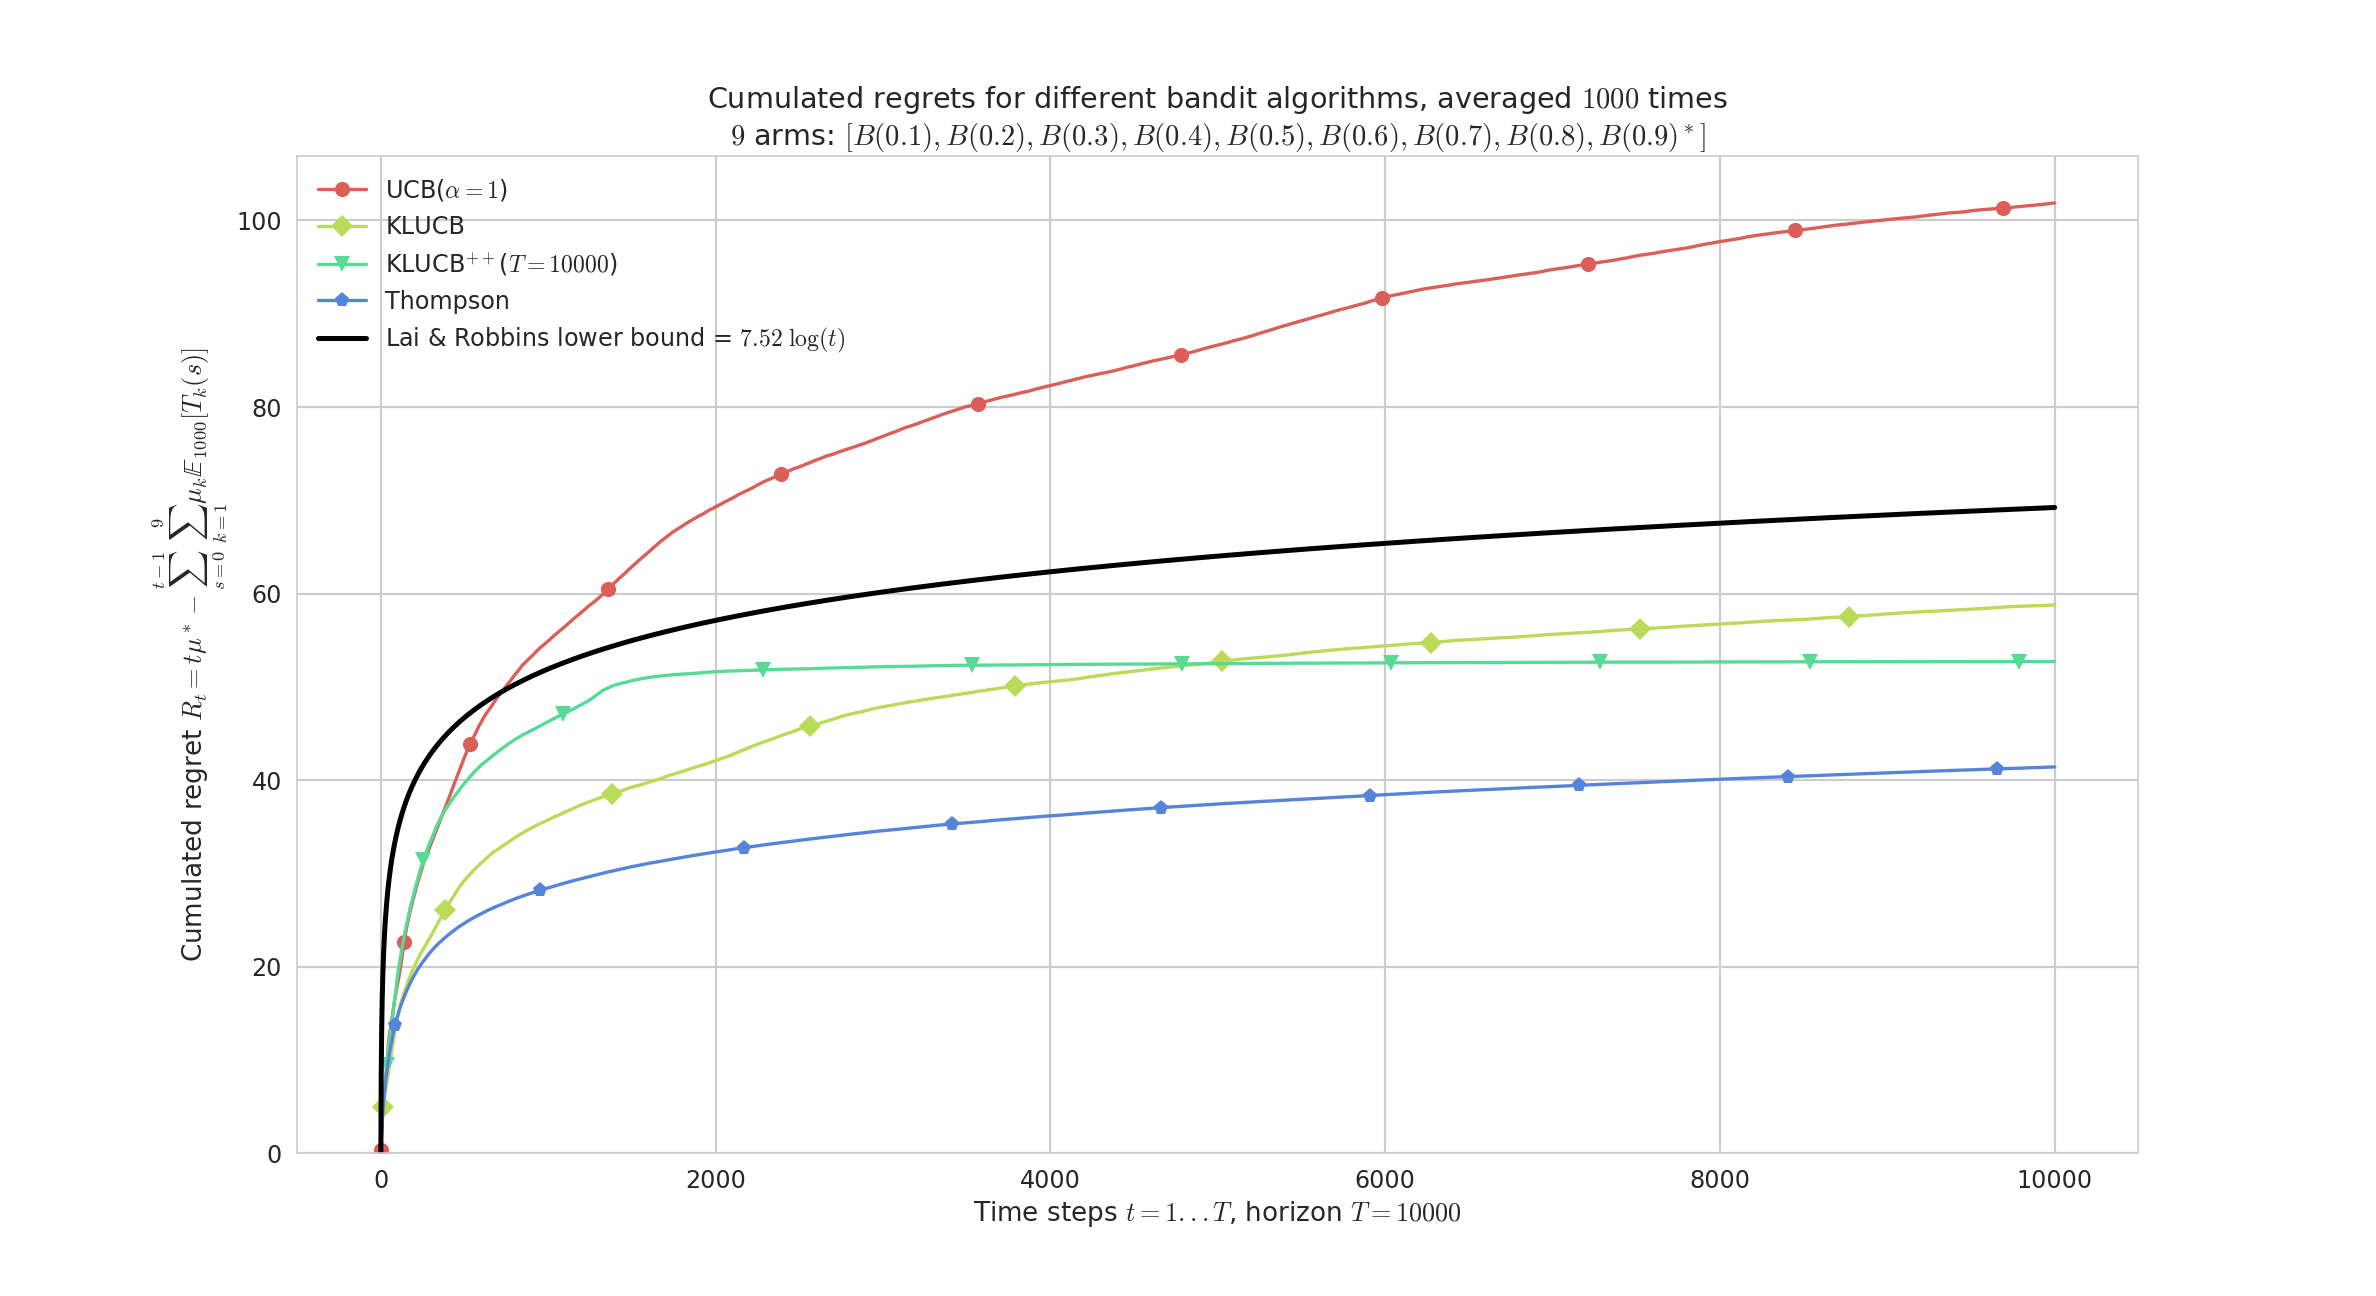
\includegraphics[width=0.95\textwidth,height=\textheight]{../plots/paper/1.png}
\caption{Single-player simulation showing the regret of \(4\)
algorithms, and the asymptotic lower-bound from {[}@LaiRobbins85{]}.
They all perform very well, and at finite time they are empirically
\emph{below} the asymptotic lower-bound. Each algorithm is known to be
order-optimal (\emph{i.e.}, its regret is proved to match the
lower-bound up-to a constant), and each but UCB is known to be optimal
(\emph{i.e.} with the constant matching the
lower-bound).\label{fig:plot1}}
\end{figure}

\begin{figure}
\centering
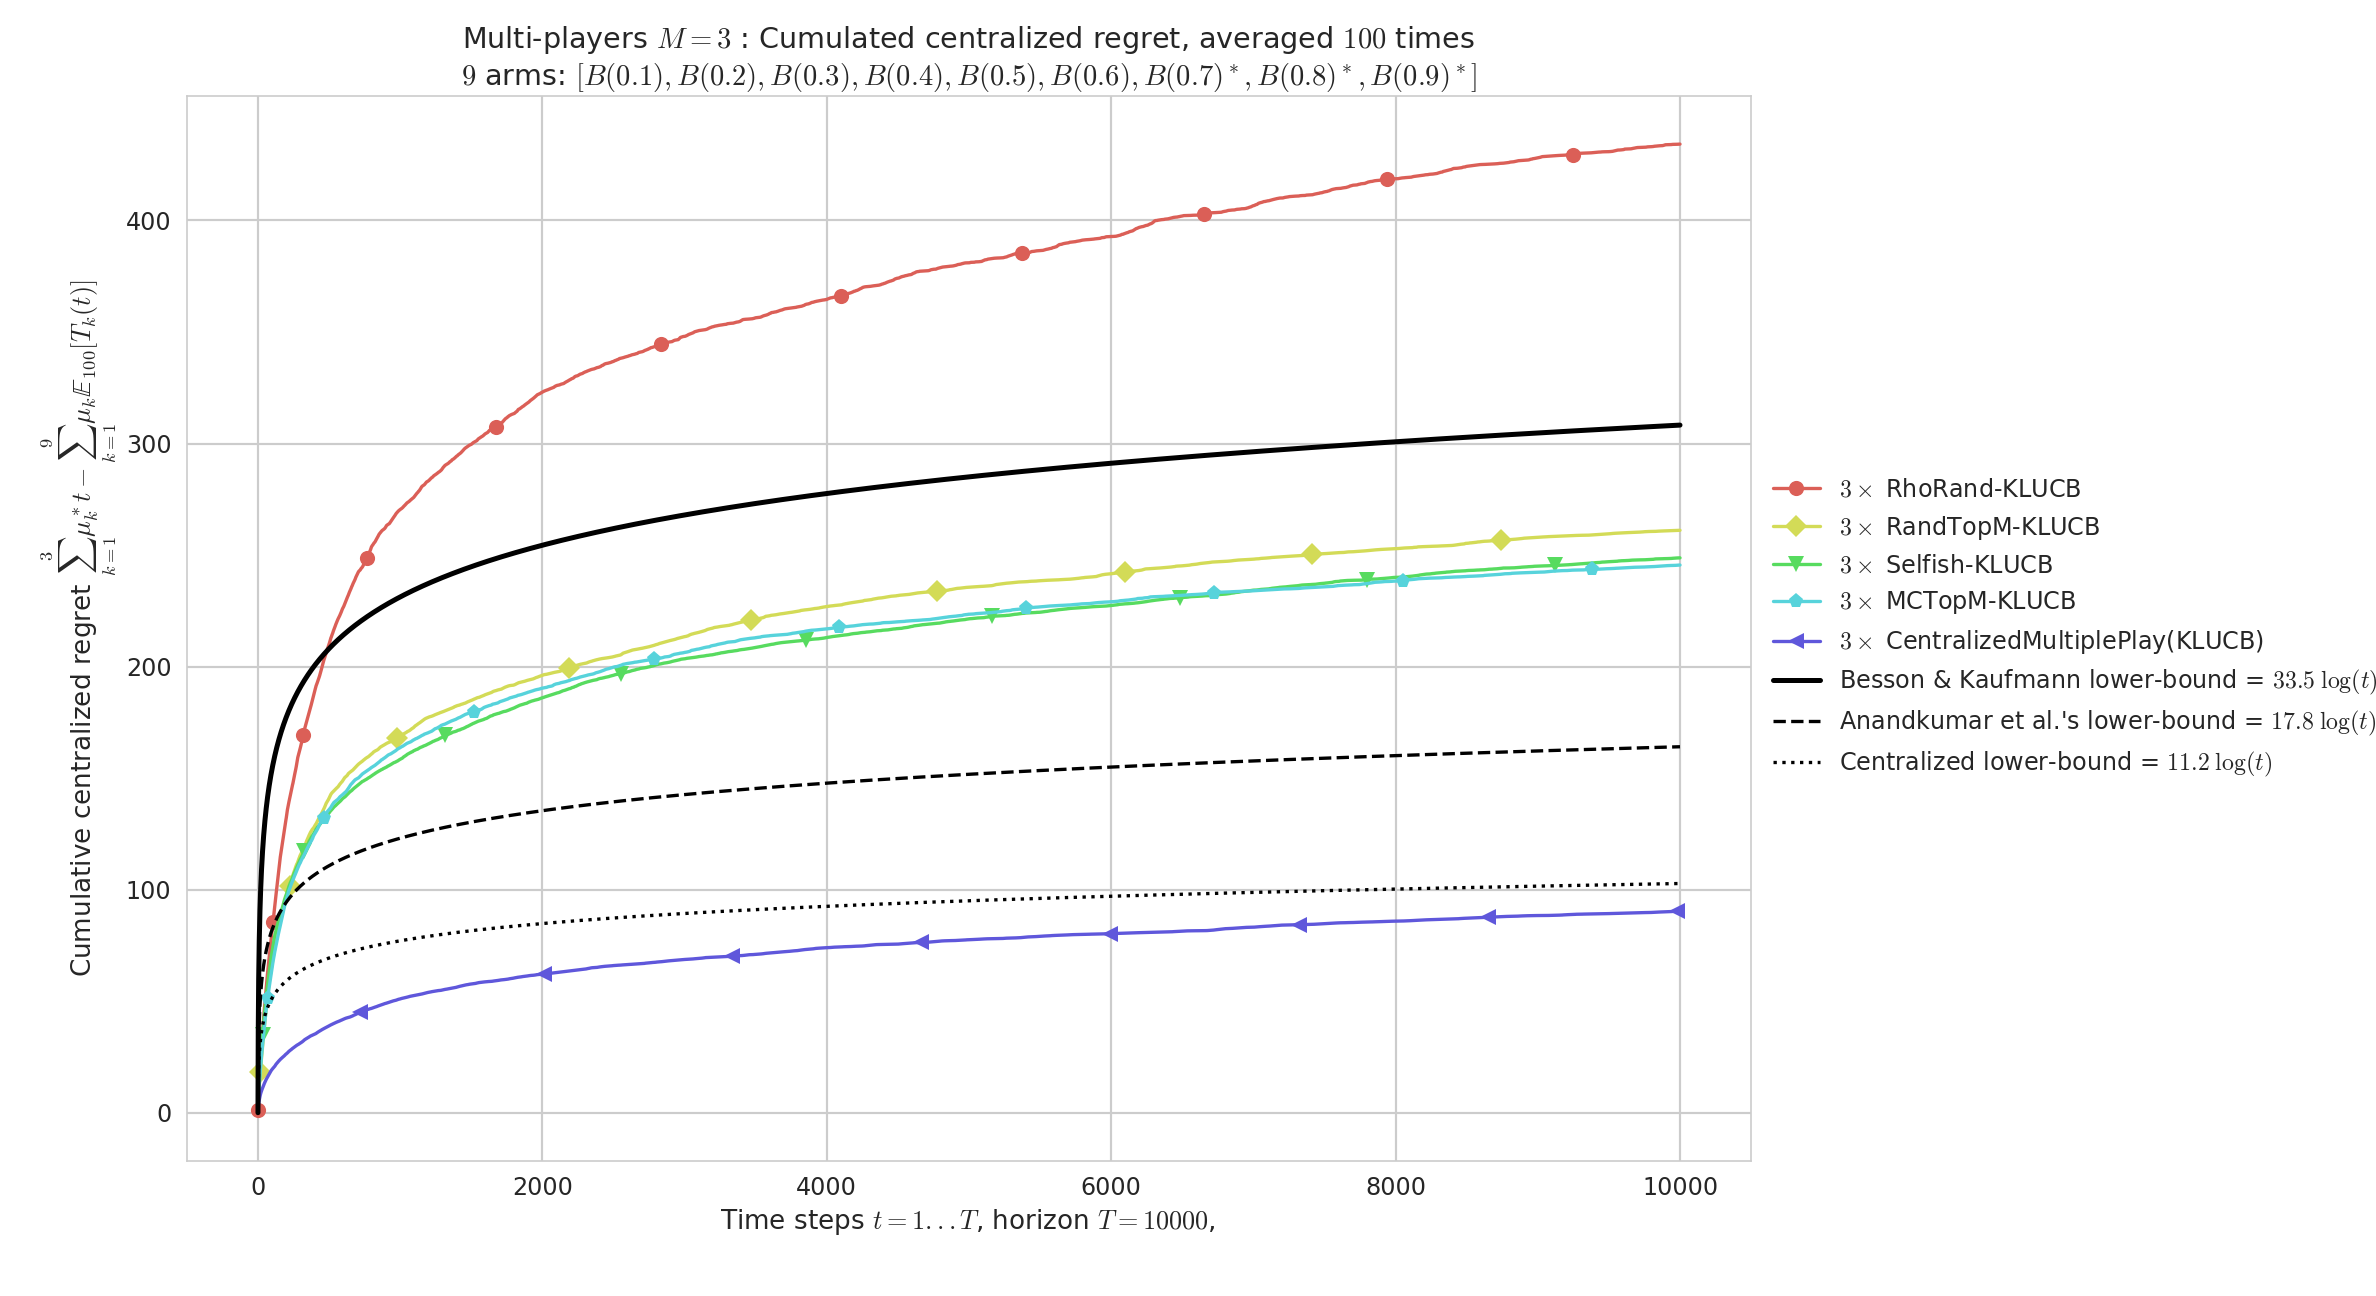
\includegraphics[width=0.95\textwidth,height=\textheight]{../plots/paper/2.png}
\caption{Multi-player simulation showing the regret of \(6\) algorithms,
and the asymptotic lower-bound from {[}@BessonALT2018{]}. The best
algorithm is the centralized version, but for decentralized algorithms,
our proposals outperform the previous state-of-the-art
\href{https://smpybandits.github.io/docs/PoliciesMultiPlayers.rhoRand.html}{\texttt{rhoRand}}
policy.\label{fig:plot2}}
\end{figure}

\begin{center}\rule{0.5\linewidth}{\linethickness}\end{center}

\hypertarget{research-using-smpybandits}{%
\subsection{\texorpdfstring{Research using
\emph{SMPyBandits}}{Research using SMPyBandits}}\label{research-using-smpybandits}}

\emph{SMPyBandits} was used for the following research articles since
\(2017\) \footnote{\href{http://perso.crans.org/besson/}{I (Lilian
  Besson)} have \href{http://perso.crans.org/besson/phd/}{started my
  PhD} in October \(2016\), and this is a part of my \textbf{on going}
  research since December \(2016\). I launched the
  \href{https://smpybandits.github.io/}{documentation} on March
  \(2017\), I wrote my first research articles using this framework in
  \(2017\) and I was finally able to open-source my project in February
  \(2018\).}:

\begin{itemize}
\item
  For this first article, {[}@Bonnefoi17{]}, \emph{SMPyBandits} was not
  used to generate the main figures, but to explore on a smaller scale
  many other approaches (using
  \href{https://smpybandits.github.io/docs/Environment.EvaluatorSparseMultiPlayers.html}{\texttt{EvaluatorSparseMultiPlayers}}).
\item
  For {[}@BessonALT2018{]}, we used \emph{SMPyBandits} for all the
  simulations for multi-player bandit algorithms \footnote{More details
    and illustrations are given on the documentation page,
    \href{https://smpybandits.github.io/MultiPlayers.html}{\texttt{MultiPlayers}}.}.
  We designed the two
  \href{https://smpybandits.github.io/docs/PoliciesMultiPlayers.RandTopM.html}{\texttt{RandTopM}}
  and
  \href{https://smpybandits.github.io/docs/PoliciesMultiPlayers.MCTopM.html}{\texttt{MCTopM}}
  algorithms and proved than they enjoy logarithmic regret in the usual
  setting, and outperform significantly the previous state-of-the-art
  solutions (\emph{i.e.},
  \href{https://smpybandits.github.io/docs/PoliciesMultiPlayers.rhoRand.html}{\texttt{rhoRand}},
  \href{https://smpybandits.github.io/docs/Policies.MEGA.html}{\texttt{MEGA}}
  and
  \href{https://smpybandits.github.io/docs/Policies.MusicalChair.html}{\texttt{MusicalChair}}).
\end{itemize}

\begin{itemize}
\tightlist
\item
  In {[}@BessonWCNC2018{]}, we used \emph{SMPyBandits} to illustrate and
  compare different aggregation algorithms \footnote{More details and
    illustrations are given on the documentation page,
    \href{https://smpybandits.github.io/Aggregation.html}{\texttt{Aggregation}}.}.
  We designed a variant of the Exp3 algorithm for online aggregation of
  experts {[}@Bubeck12{]}, called
  \href{https://smpybandits.github.io/docs/Policies.Aggregator.html}{\texttt{Aggregator}}.
  Aggregating experts is a well-studied idea in sequential learning and
  in machine learning in general. We showed that it can be used in
  practice to select on the run the best bandit algorithm for a certain
  problem from a fixed pool of experts. This idea and algorithm can have
  interesting impact for Opportunistic Spectrum Access applications
  {[}@Jouini09{]} that use multi-armed bandits algorithms for sequential
  learning and network efficiency optimization.
\end{itemize}

\begin{itemize}
\tightlist
\item
  In {[}@Besson2018c{]}, we used \emph{SMPyBandits} to illustrate and
  compare different ``doubling trick'' schemes \footnote{More details
    and illustrations are given on the documentation page,
    \href{https://smpybandits.github.io/DoublingTrick.html}{\texttt{DoublingTrick}}.}.
  In sequential learning, an algorithm is \emph{anytime} if it does not
  need to know the horizon \(T\) of the experiments. A well-known trick
  for transforming any non-anytime algorithm to an anytime variant is
  the ``Doubling Trick'': start with a horizon \(T_0\in\mathbb{N}\),
  and when \(t > T_i\), use \(T_{i+1} = 2 T_i\). We studied two generic
  sequences of growing horizons (geometric and exponential), and we
  proved two theorems that generalized previous results. A geometric
  sequence suffices to minimax regret bounds (in
  \(R_T = \mathcal{O}(\sqrt(T))\)), with a constant multiplicative loss
  \(\ell \leq 4\), but cannot be used to conserve a logarithmic regret
  bound (in \(R_T = \mathcal{O}(\log(T))\)). And an exponential sequence
  can be used to conserve logarithmic bounds, with a constant
  multiplicative loss also \(\ell \leq 4\) in the usual setting. It is
  still an open question to know if a well-tuned exponential sequence
  can conserve minimax bounds or weak minimax bounds (in
  \(R_T = \mathcal{O}(\sqrt{T \log(T)})\)).
\end{itemize}

\hypertarget{dependencies}{%
\subsection{Dependencies}\label{dependencies}}

The framework is written in Python {[}@python{]}, using matplotlib
{[}@matplotlib{]} for 2D plotting, numpy {[}@numpy{]} for data storing,
random number generations and operations on arrays, scipy
{[}@scipy{]} for statistical and special functions, and seaborn
{[}@seaborn{]} for pretty plotting and colorblind-aware colormaps.
Optional dependencies include joblib {[}@joblib{]} for parallel
simulations, numba {[}@numba{]} for automatic speed-up on some small
functions, as well as sphinx {[}@sphinx{]} for generating the
documentations. I also acknowledge the use of virtualenv
{[}@virtualenv{]} for launching simulations in isolated environments,
and jupyter {[}@jupyter{]} used with ipython {[}@ipython{]} to
experiment with the code.

\begin{center}\rule{0.5\linewidth}{\linethickness}\end{center}
